Per valutare e quantificare la capacità di generalizzazione Out-of-Distribution (OOD) del modello analizzato in questo progetto, abbiamo strutturato i test utilizzando tre dataset della famiglia ImageNet. In particolare, abbiamo utilizzato i dataset ImageNet-1k, ImageNet-C e ImageNet-R.
In questo capitolo, descriveremo le caratteristiche principali di ciascun dataset e le motivazioni che ci hanno portato a sceglierli per i nostri test.
\section{ImageNet}
ImageNet è un ampio dataset d'immagini etichettate, ampiamente utilizzato per addestrare e valutare modelli di visione artificiale. Contiene oltre 14 milioni d'immagini annotate con più di 20.000 categorie di oggetti.
La costruzione del dataset è stata effettuata in tre fasi:
\begin{enumerate}
	\item \textbf{Mappatura WordNet}: per strutturare il dataset è stata usata la struttura gerarchica di WordNet, un database lessicale che organizza le parole in insiemi di sinonimi (synsets) e le collega tra loro attraverso relazioni semantiche. Ogni synset ha un "WordNet ID" (WNID) univoco, che è stato utilizzato per etichettare le immagini nel dataset. In questo modo, le immagini sono state organizzate in categorie gerarchiche basate sui synset di WordNet.
	\item \textbf{Web scraping}: le immagini sono state raccolte da Internet utilizzando tecniche di web scraping. Sono stati utilizzati motori di ricerca e altre fonti online per raccogliere immagini pertinenti alle categorie di oggetti definite dai synset di WordNet.
	\item \textbf{Annotazione manuale}: le immagini raccolte sono state annotate manualmente attraverso il servizio Amazon Mechanical Turk(AMTurk). Ogni immagine è stata etichettata con la categoria di oggetti corretta, garantendo così l'accuratezza delle annotazioni.
\end{enumerate}
Il database completo originario è noto come ImageNet-21K (o ImageNet-22K) e contiene circa 14,2 milioni d'immagini distribuite su 21.841 classi gerarchiche. Non è presente uno split training-validation-test ufficiale. Il dataset non è bilanciato: alcune classi contengono un numero molto basso di esempi, mentre altre classi contengono un numero elevato di esempi.
\section{ImageNet-1k}
Vengono spesso utilizzati subset di ImageNet-21k per vari scopi. 
Uno dei più noti è ImageNet-1k, che contiene 1.000 classi di oggetti selezionate da ImageNet-21k. Il dataset contiene 1.281.167 immagini di training, 50.000 immagini (50 per classe) di validation e 100.000 immagini di test.

Questo dataset è stato utilizzato per addestrare e valutare modelli di visione artificiale, in particolare per la competizione ImageNet Large Scale Visual Recognition Challenge (ILSVRC). Per questo motivo, il test set non è etichettato, in quanto serve unicamente a valutare le prestazioni dei modelli durante la competizione. Perciò, per i nostri test, abbiamo utilizzato il validation set come test set, questo è possibile in quanto il validation set non viene utilizzato per l'addestramento del modello, ma solo per la valutazione delle sue prestazioni\cite{he_deep_2016}.

A differenza della struttura gerarchica ad albero di ImageNet-21K (che include macro-classi come "mammifero" o "veicolo"), ImageNet-1K contiene esclusivamente 1.000 classi non sovrapposte poste alla base dell'albero gerarchico (es. singole razze di cani come "German shepherd", senza includere la classe genitore "dog")
\section{ImageNet-C}
A differenza di altri dataset, ImageNet-C non è stato raccolto fotografando nuovi oggetti o facendo web scraping. È stato costruito applicando sistematicamente corruzioni digitali e matematiche direttamente sul set di validazione originale di ImageNet-1K (le 50.000 immagini di validazione)
L'obiettivo dei creatori era imitare le reali limitazioni fisiche dei sensori delle fotocamere, le variazioni atmosferiche ambientali e i disturbi dovuti alla compressione e trasmissione dei dati, escludendo però alterazioni avversariali mirate (worst-case)\cite{hendrycks_benchmarking_2019}.
Il dataset si sviluppa in modo gerarchico:
\begin{itemize}
	\item \textbf{Corruzioni}: sono state applicate 15 corruzioni digitali e matematiche, suddivise in 4 categorie principali: \textit{blur}, \textit{noise}, \textit{digital} e \textit{weather}. 
	\begin{itemize}
		\item \textit{Blur}: motion blur, defocus blur, frosted glass blur, gaussian blur, zoom blur
		\item \textit{Noise}: gaussian noise, shot noise, impulse noise
		\item \textit{Digital}: brightness, contrast, elastic transform, pixelate, jpeg compression
		\item \textit{Weather}: snow, frost, fog
	\end{itemize}
	\item \textbf{Intensità}: per ogni corruzione sono stati generati 5 livelli di intensità, da 1 (minima) a 5 (massima).
\end{itemize}
La dimensione totale del test set di ImageNet-C è quindi di $50.000 \times 15 \text{ corruzioni} \times 5 \text{ severità} = 3.750.000$ immagini di test.
\begin{figure}[H]
	\centering
	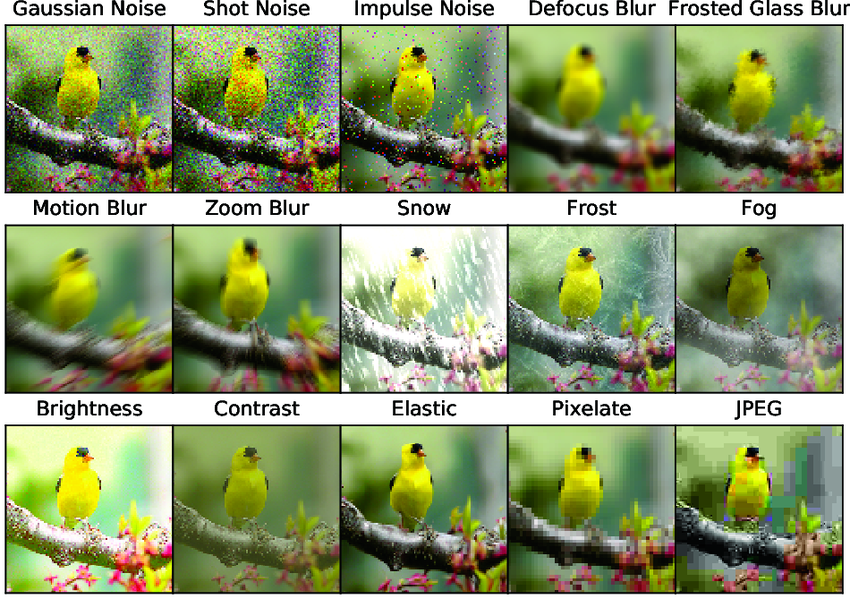
\includegraphics[width=0.8\textwidth]{images/ImageNetC_example.png}
	\caption{Esempi di corruzioni applicate a un'immagine del dataset ImageNet-1K.}
	\label{fig:imagenet_c}
\end{figure}
\section{ImageNet-R}
ImageNet-R è un dataset di immagini raccolte da Internet, progettato per testare la capacità di generalizzazione dei modelli di visione artificiale su immagini stilizzate e artistiche. Il dataset è stato creato seguendo le seguenti procedure descritte in \cite{hendrycks_many_2021}:
\begin{enumerate}
	\item \textbf{Sottocampionamento delle classi}: Gli autori hanno selezionato un subset di 200 classi di ImageNet-1K. Ciò è stato necessario a causa della difficoltà di trovare immagini stilizzate per tutte le 1.000 classi di ImageNet-1K, dunque sono state selezionate solo le classi per le quali era possibile reperire un numero sufficiente d'immagini stilizzate. Inoltre sono state scelte classi facilmente riconoscibili da un umano, ad esempio "cane" invece che indicare una razza specifica di cane.
	\item \textbf{Raccolta delle immagini}: Le immagini sono state ottenute tramite scraping da Flickr, fonte da cui erano state ottenute parte delle immagini di ImageNet-1K. 
	\item \textbf{Filtro di Qualità Manuale}:

    \begin{itemize}
		\item I lavoratori di Amazon Mechanical Turk hanno eseguito una prima scrematura scartando i falsi positivi (immagini non coerenti con la classe semantica cercata).
		\item Un team di studenti di dottorato ha eseguito una revisione manuale finale, eliminando le immagini con etichette ambigue o multiple per garantire che ogni immagine avesse un'unica classe definita e corretta
	\end{itemize} 
\end{enumerate}
Il dataset finale contiene 30.000 immagini di test, con un numero variabile d' immagini per classe, da un minimo di 51 a un massimo di 430 immagini per classe, in media 150 immagini per classe.
Le immagini sono categorizzate in base a diversi stili (es. Painting, Sculpture, Origami, Cartoon, Toy, Embroidery, ecc.). Ai fini della classificazione, le etichette di destinazione rimangono quelle semantiche di ImageNet-1K.
\begin{figure}[H]
	\centering
	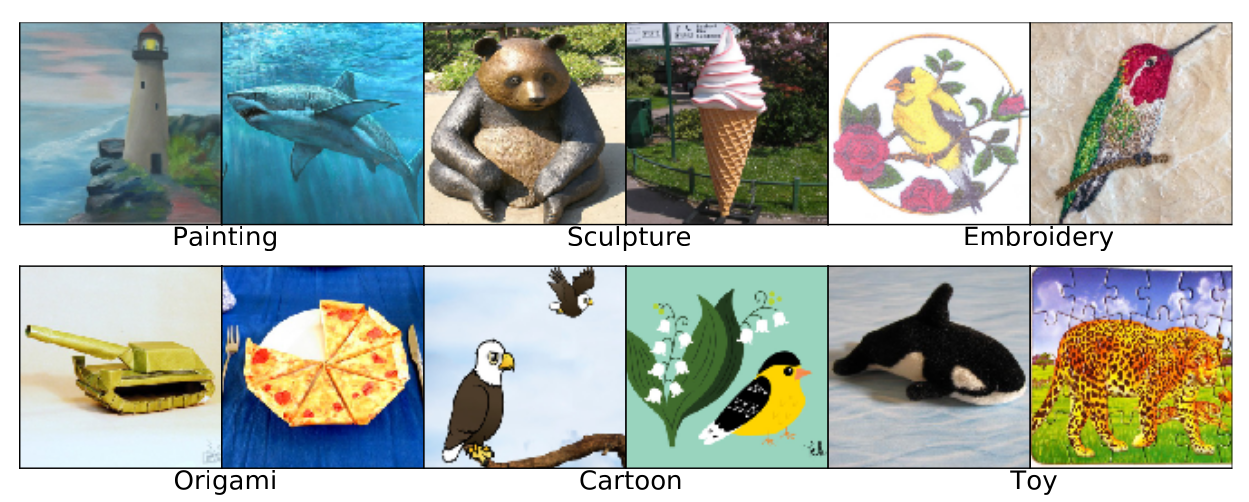
\includegraphics[width=0.8\textwidth]{images/ImageNetR_example.png}
	\caption{Esempi di immagini stilizzate del dataset ImageNet-R. Painting, etc. sono stili di rappresentazione, non etichette.}
	\label{fig:imagenet_r}
\end{figure}